\documentclass[fleqn]{article}
\usepackage[spanish]{babel}
\usepackage{amsmath}
\usepackage{amsthm}
\usepackage{graphicx}
\usepackage[utf8]{inputenc}

%%%%%%%% MARGIN
\usepackage[left=1in, right=1in, top=0.8in, bottom=0.8in]{geometry}

%%%%%%%% NO PARAGRAPH INDENT
% https://tex.stackexchange.com/questions/27802/set-noindent-for-entire-file
\setlength\parindent{0pt}

%%%%%%%% SUB-FIGURE PACKAGE
\usepackage{subcaption}

%%%%%%%% HYPERREF PACKAGE
\usepackage{hyperref}
\hypersetup{linkcolor=blue}
\hypersetup{citecolor=blue}
\hypersetup{urlcolor=blue}
\hypersetup{colorlinks=true}

%%%%%%%% MULTI-COLUMNS PACKAGE
\usepackage{multicol}

%%%%%%%% SETS DEFINITIONS
\usepackage{amssymb}
%%%% Important sets
\renewcommand{\O}{\mathbb{O}}
\newcommand{\N}{\mathbb{N}}
\newcommand{\Z}{{\mathbb{Z}}}
\newcommand{\Q}{{\mathbb{Q}}}
\newcommand{\R}{{\mathbb{R}}}

%%%% Statistics
\newcommand{\E}[1]{\mathbb{E}\left[#1 \right]}
\newcommand{\V}[1]{\mathrm{Var}\left[#1 \right]}

%%%% Lambda Calculus Symbols
\newcommand{\dneq}{\,\, \# \,\,}
\renewcommand{\S}{\pmb{\mathrm{S}}}
\newcommand{\I}{\pmb{\mathrm{I}}}
\newcommand{\K}{\pmb{\mathrm{K}}}
\newcommand{\ch}[1]{\ulcorner #1 \urcorner}

%%%% Ordinal Lambda Calculus Symbols
\newcommand{\ordAlph}{\Sigma_{\text{Ord}}}
\newcommand{\termOrd}{\text{Term}_\text{Ord}}
\newcommand{\fl}{\mathrm{fl}}
\newcommand{\sk}{\mathrm{sk}}

%%%% Superscript to the left
% https://latex.org/forum/viewtopic.php?t=455
\usepackage{tensor}
\newcommand{\app}[3]{\tensor*[^{#1}]{\left(#2, #3\right)}{}}

%%%% Make optional parameter
% https://tex.stackexchange.com/questions/217757/special-behavior-if-optional-argument-is-not-passed
\usepackage{xparse}
\NewDocumentCommand{\cx}{o}{
  \IfNoValueTF{#1}
  {\left[\quad\right]}
  {\left[\, #1 \,\right]}
}

%%%%%%%% LOGIC TREES
\usepackage{prftree}

%%%%%%%% SPLIT EQUATIONS
% https://tex.stackexchange.com/questions/51682/is-it-possible-to-pagebreak-aligned-equations
\allowdisplaybreaks

%%%%%%%% CODE RENDERING
% Compile with flag -shell-escape
\usepackage{minted}
\usemintedstyle{vs}

%%%%%%%% EXAM PACKAGE
\usepackage{mathexam}

%%%%%%%% CHANGE MARGINS ITEMIZE
\usepackage{enumitem}

%%%%%%%% START DOCUMENT

\ExamClass{ÁLGEBRA EN C.d.l.D}
\ExamName{EXAMEN 1}
\ExamHead{\today}

\let\ds\displaystyle

\begin{document}
 \vspace{0.3cm}
   % Information of the student
   \begin{itemize}[leftmargin=6.25cm, labelsep=0.5cm]

     \item[\textit{Nombre}] \scalebox{1.2}{Juan Sebastián Cárdenas Rodríguez} % Name
     \item[\textit{Código}] 201710008101 % Code

   \end{itemize}
\vspace{0.3cm}

% Each of the items to solve
\begin{enumerate}
  \item Solución a cada item.
    \begin{enumerate}
      \item Solución al a) y al b):
      \begin{figure}[H]
        \centering
        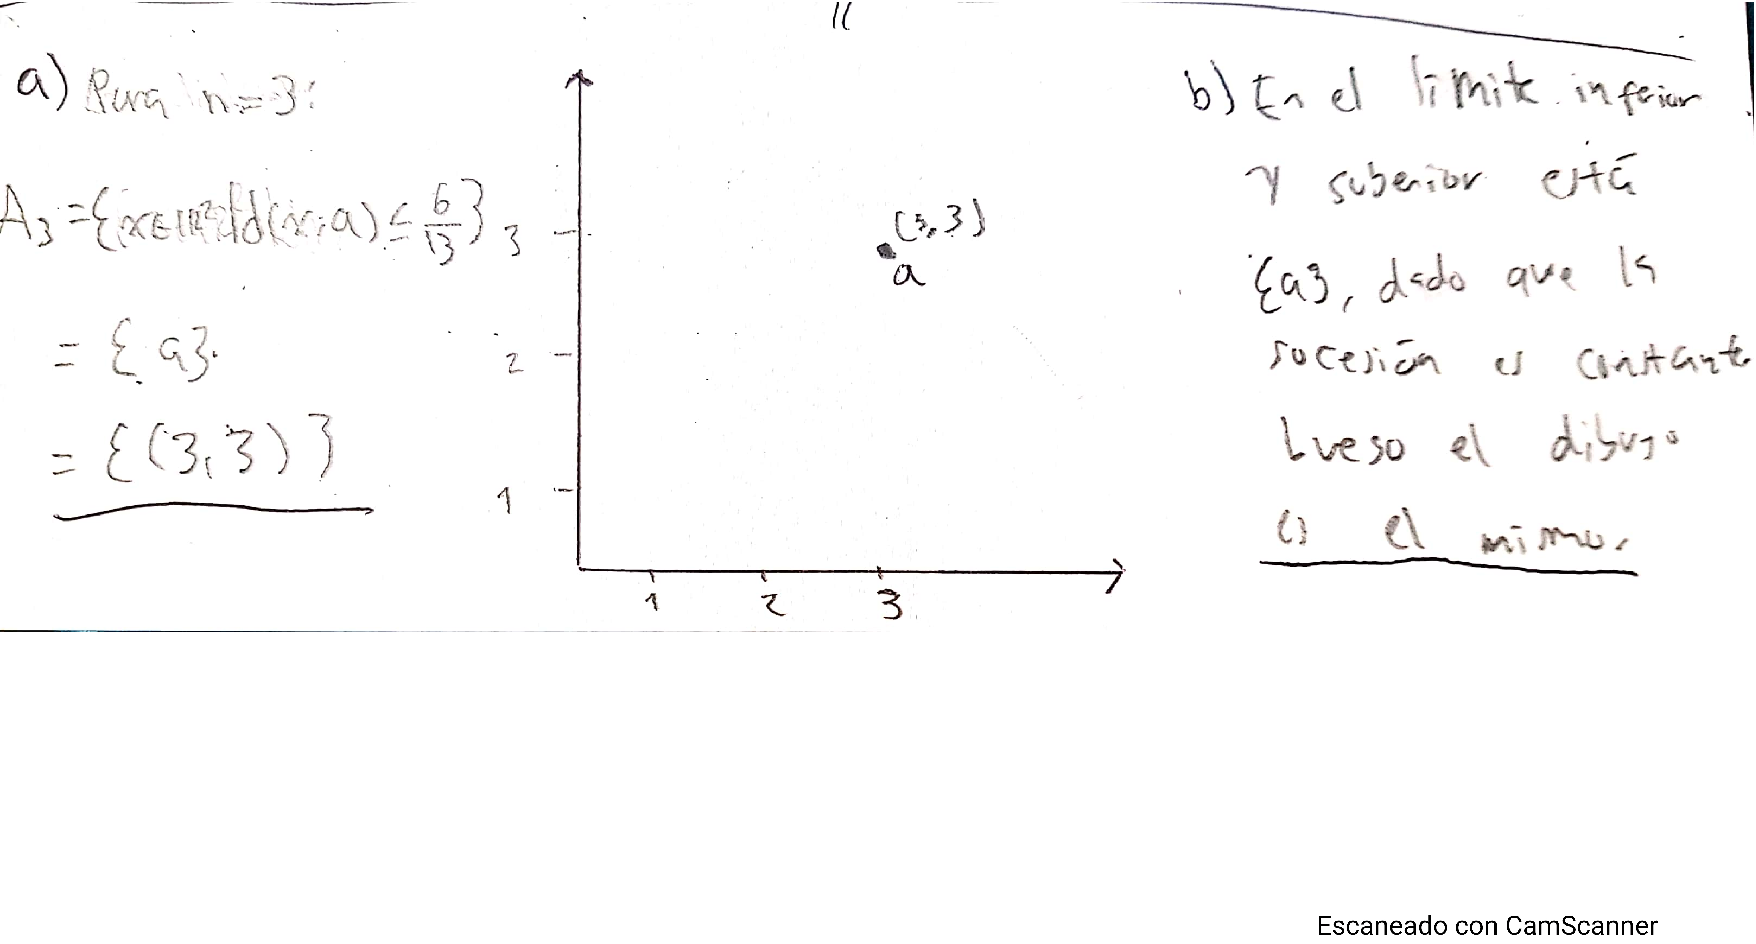
\includegraphics[scale=.4]{figs/1ab}
      \end{figure}
      \item Solución al ítem c):
      \begin{figure}[H]
        \centering
        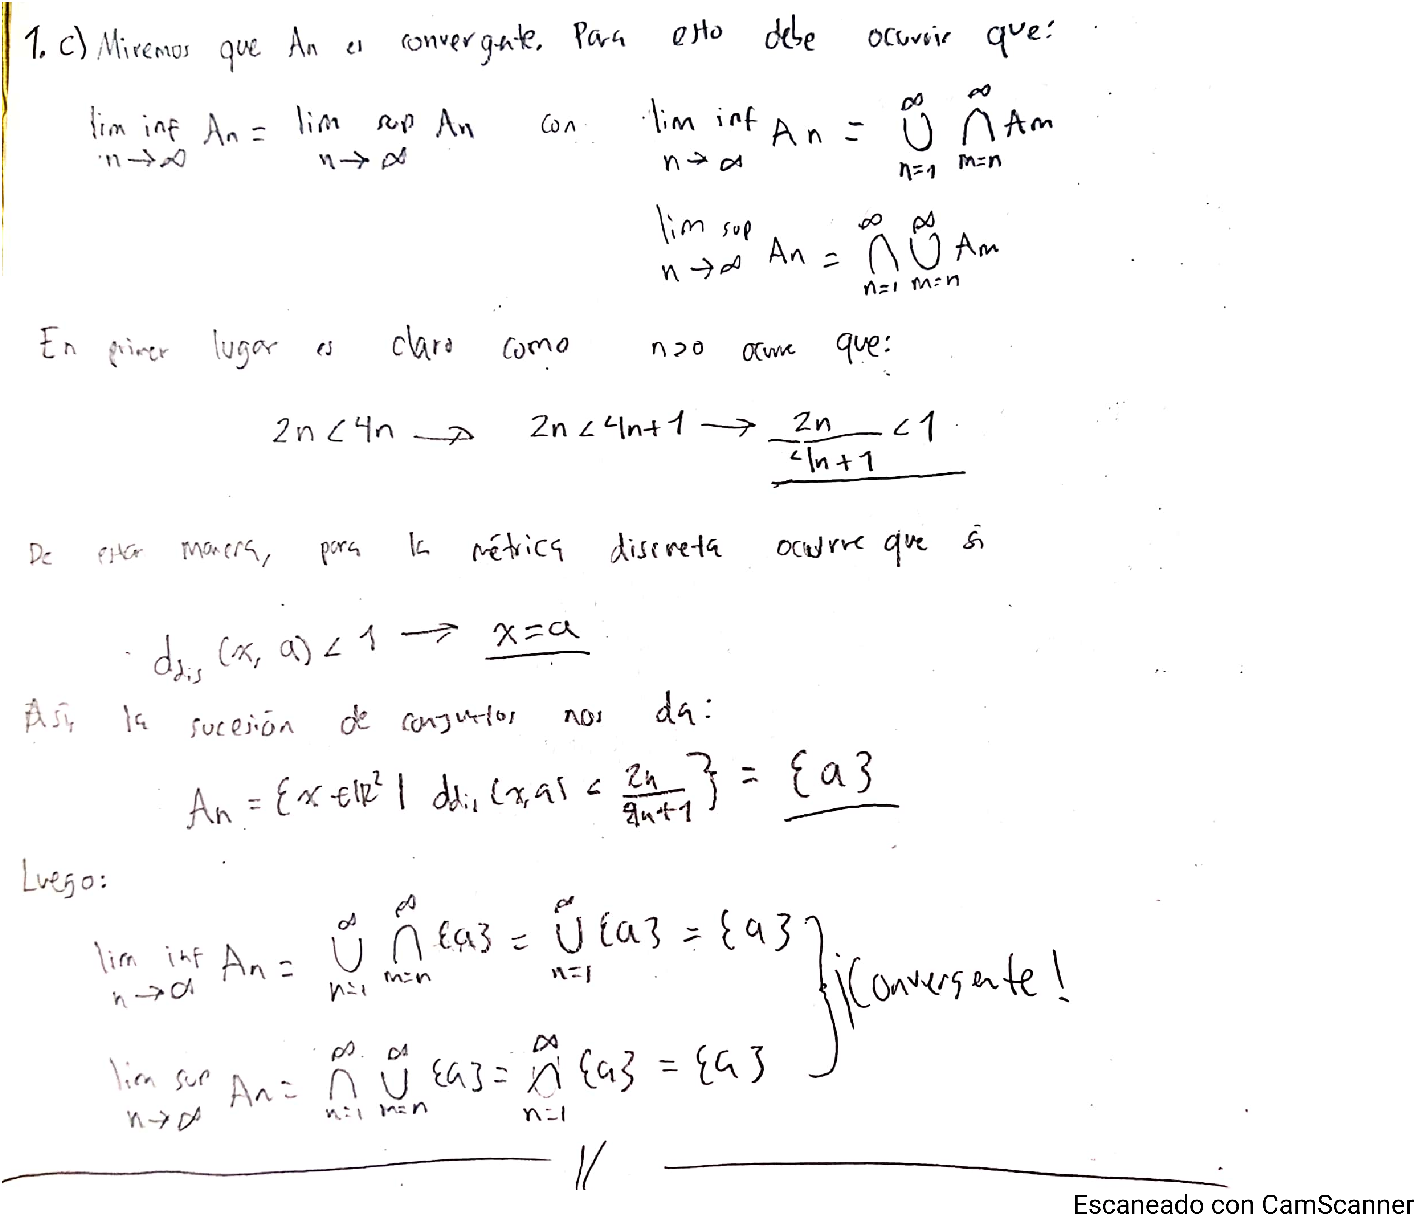
\includegraphics[scale=.5]{figs/1c}
      \end{figure}
    \end{enumerate}
    \newpage

  \item Solución:
    \begin{figure}[H]
      \centering 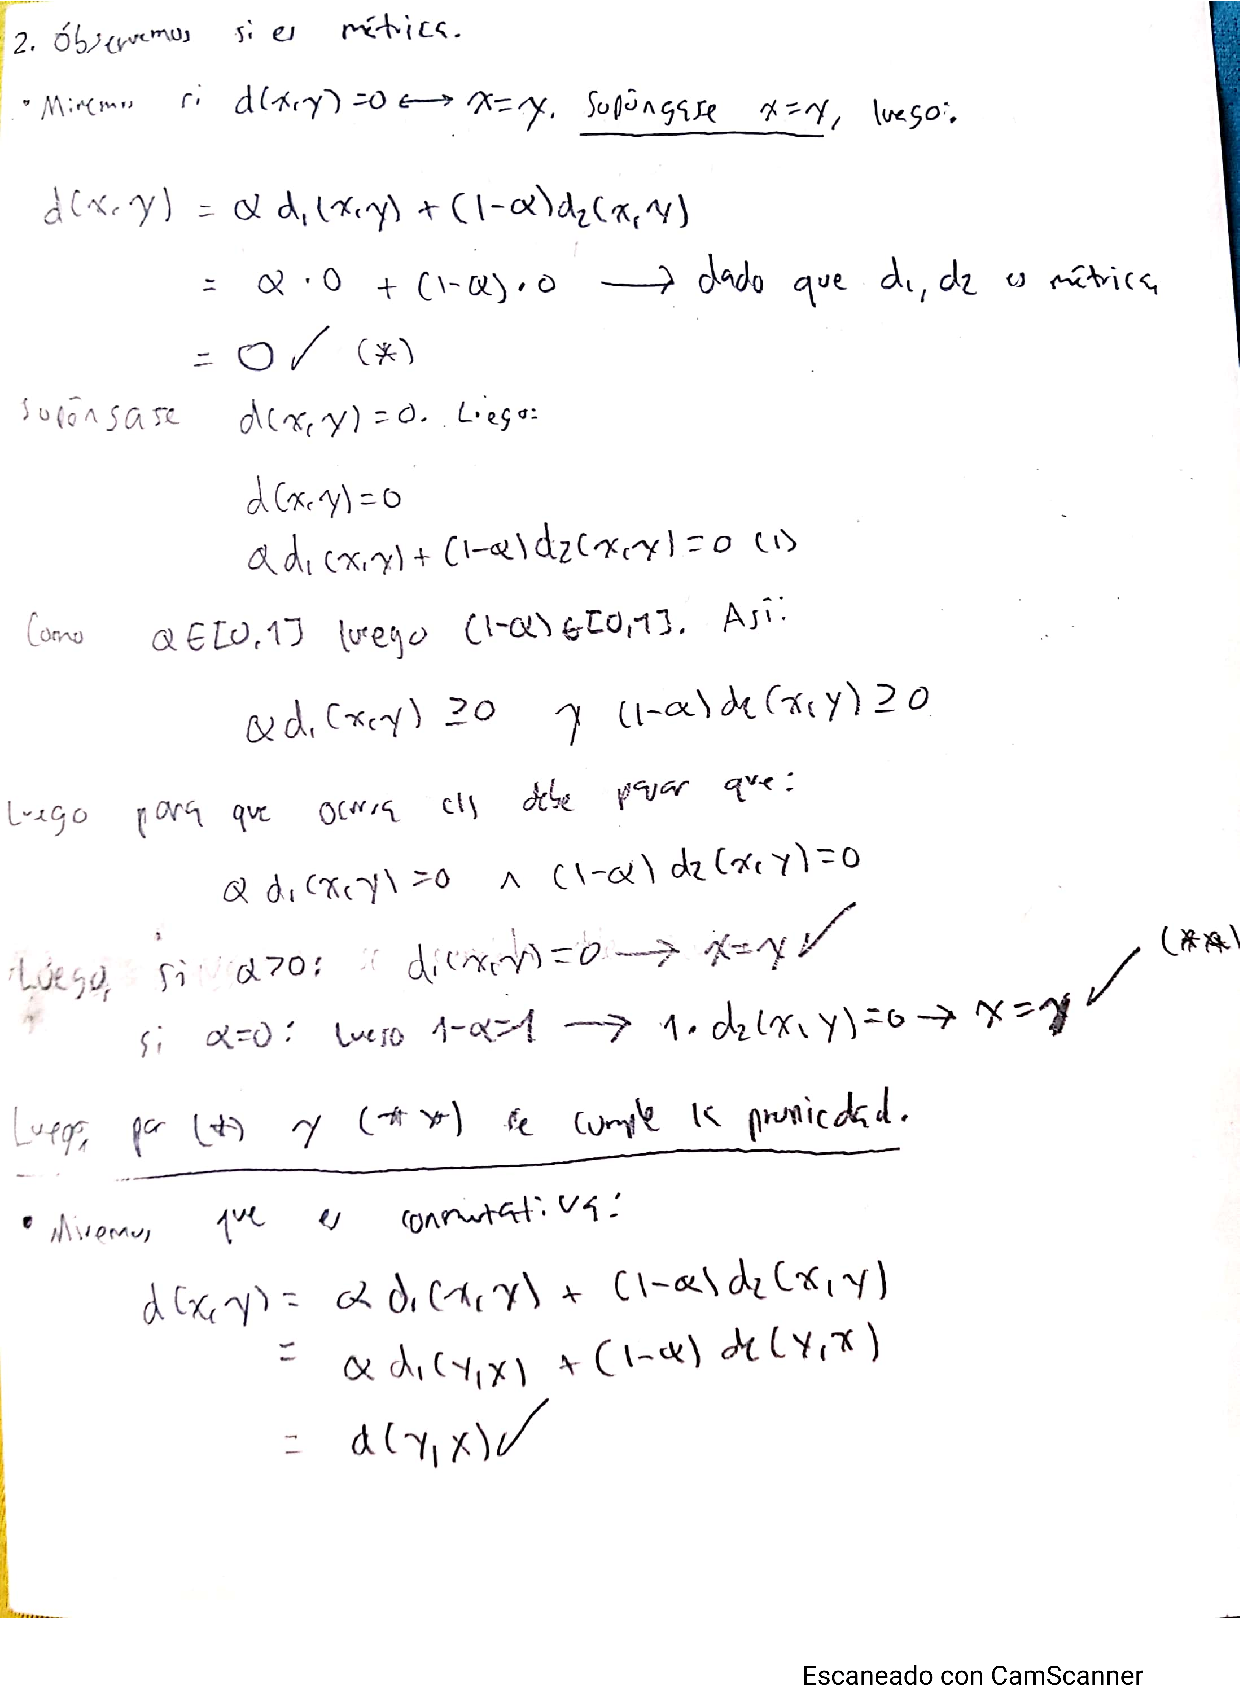
\includegraphics[scale=.8]{figs/2a}
    \end{figure}
    \begin{figure}[H]
      \centering 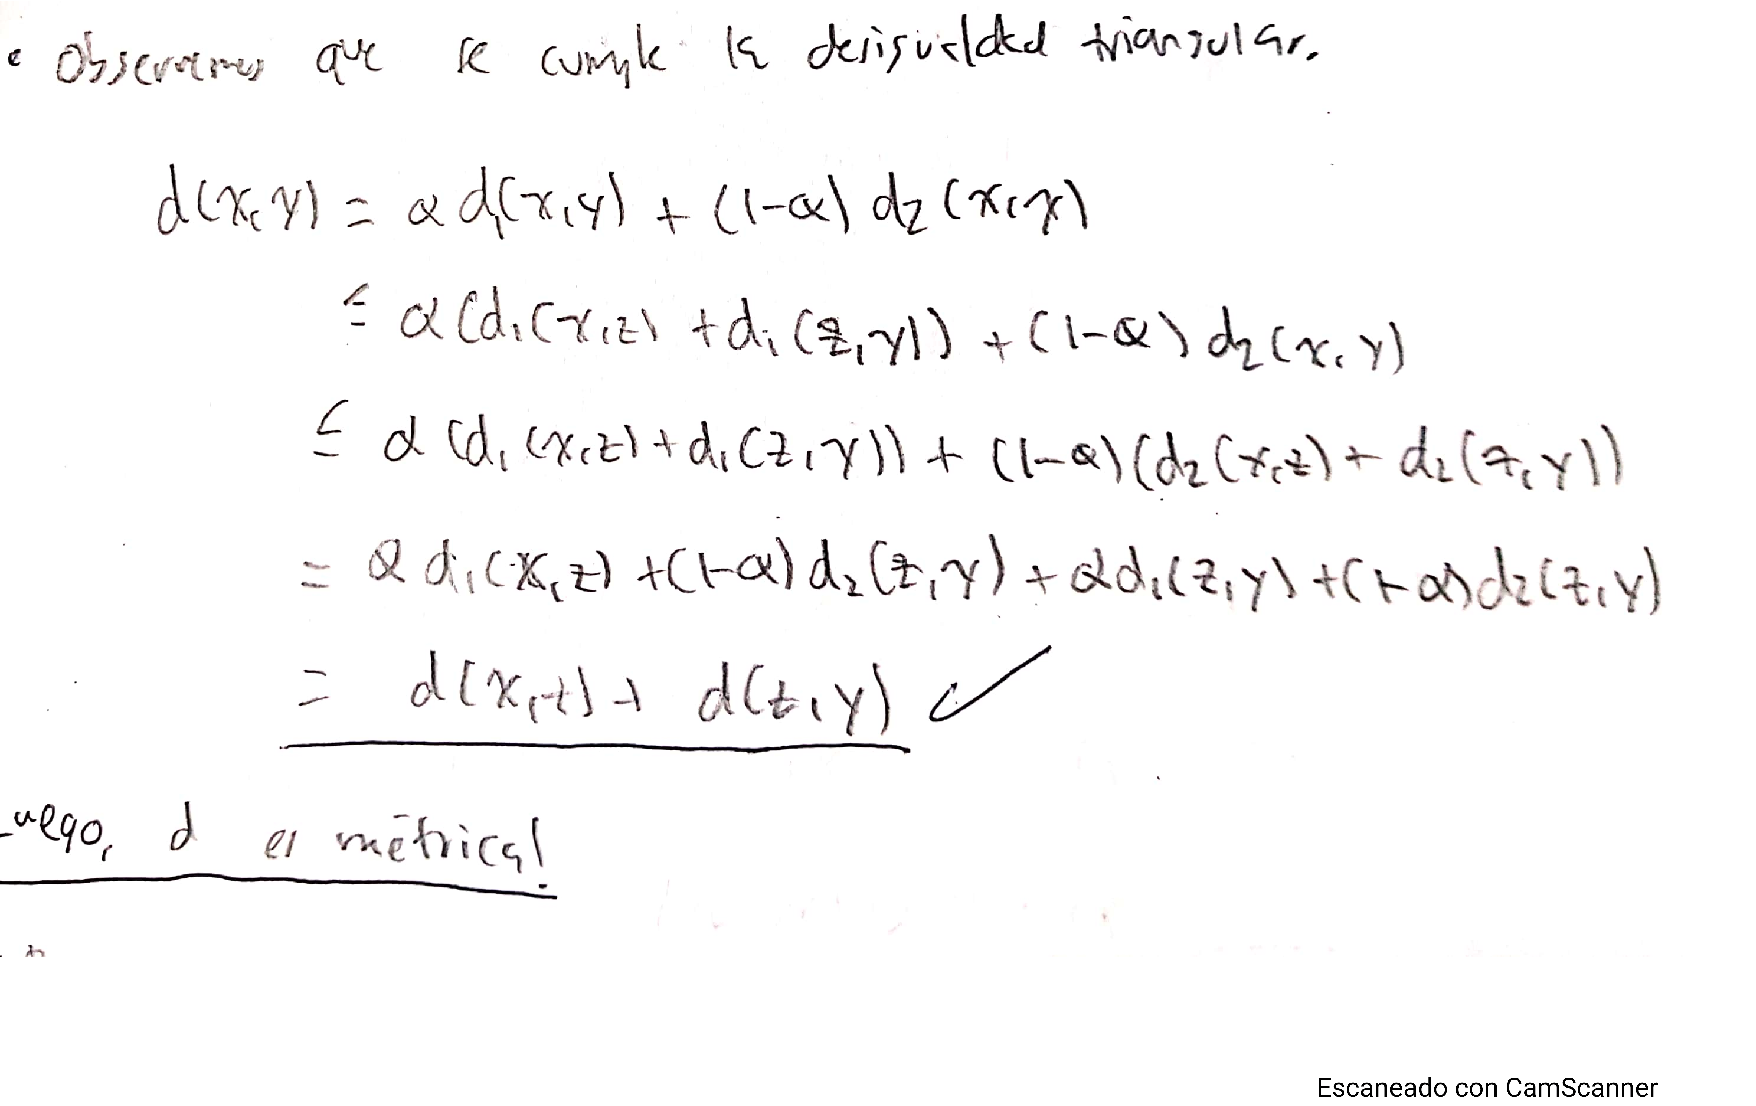
\includegraphics[scale=.5]{figs/2b}
    \end{figure}
    \begin{figure}[H]
      \centering 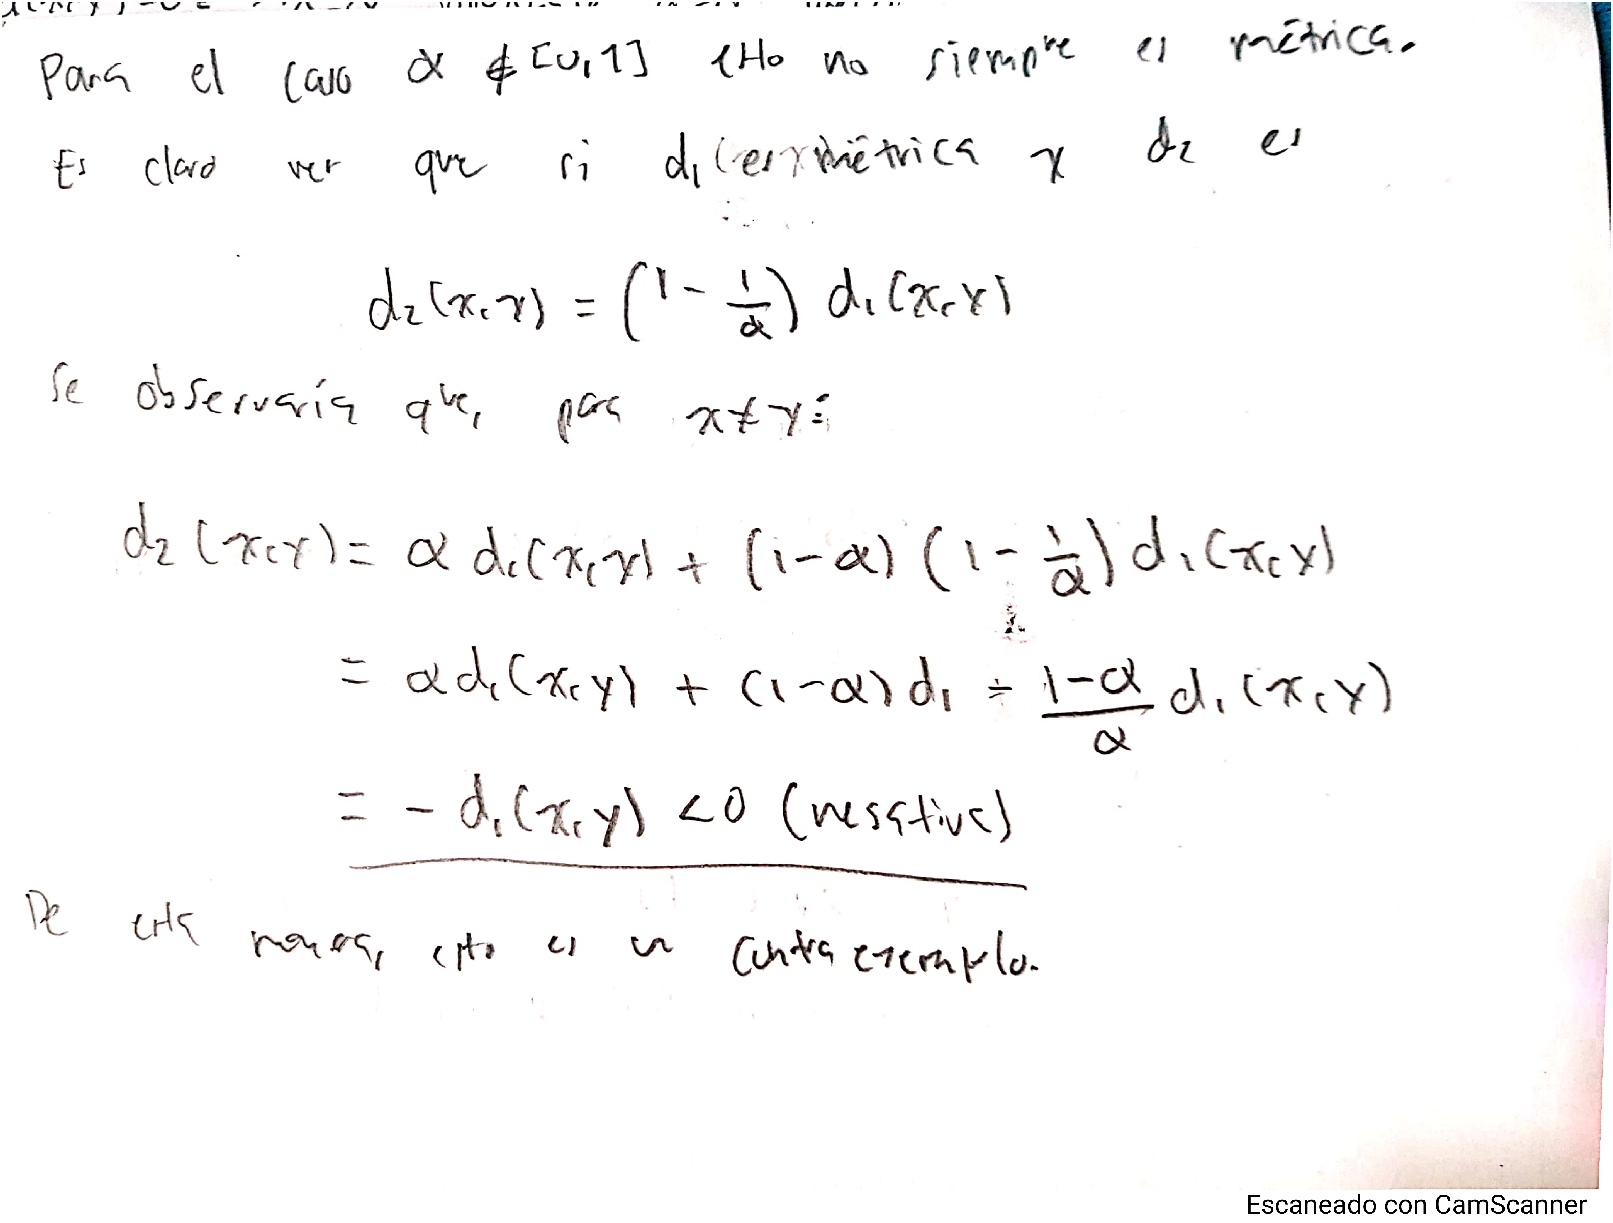
\includegraphics[scale=.5]{figs/2c}
    \end{figure}
    \newpage

    \item Código: \inputminted[firstline=1, lastline=37]{python}{src/exam.py}

    El resultado de este código nos muestra la gráfica pedida por el ejercicio
    así:
    \begin{figure}[H]
      \centering
      \includegraphics[scale=.5]{src/hilbert_distance}
    \end{figure}

    En primer lugar, se observa que no hay un error mayor entre ambas
    soluciones. Esto se da precisamente porque la librería \texttt{numpy} tiene
    métodos auxiliares que ayudan a tratar matrices mal condicionadas. Sin
    embargo, se puede observar que la distancia no es 0 que sería lo ideal.

    Esto ocurre porque la matriz de Hilbert está mal condicionada, de esta
    manera afectando que la solución sea exacta. Para solucionar esto, saquemos
    la pseudo inversa. Código: \inputminted[firstline=39,
    lastline=52]{python}{src/exam.py}

    Sacando la pseudo-inversa, obtenemos la siguiente gráfica de distancias:
    \begin{figure}[H]
      \centering
      \includegraphics[scale=.5]{src/hilbert_distance_pseudo}
    \end{figure}

    Se observa que claramente esta mejora la distancia a la solución real.

  \item Código: \inputminted[firstline=54, lastline=76]{python}{src/exam.py}

    Este código genera la gráfica para el número de condición dado n:
    \begin{figure}[H]
      \centering \includegraphics[scale=.5]{src/cond_b}
    \end{figure}

    Es claro que a medida que se va incrementando $n$ el número de condición va
    aumentando drásticamente. Esto es porque a medida que $n$ se incrementa, la
    matriz cada vez está más cerca de ser una matriz no-invertible sin llegar a
    serlo. De esta manera, generando más error.

    El código para lo de Ledoit Wolf es: \inputminted[firstline=79,
    lastline=98]{python}{src/exam.py}

    Óbservese la gráfica del número de condición y el determinante.
    \begin{figure}[H]
      \centering
      \begin{subfigure}[b]{0.45\textwidth}
        \centering \includegraphics[scale=.4]{src/cond_b_lw}
        \caption{Número de condición.}
      \end{subfigure}
      %
      \begin{subfigure}[b]{0.45\textwidth}
        \centering \includegraphics[scale=.4]{src/det_lw}
        \caption{Determinante.}
      \end{subfigure}
    \end{figure}

    Para esto, se generaron valores de una normal multivariada con covarianza
    $B_{n}$ y se guardó en $D_{n}$. De esta manera, se puede observar como
    Ledoit-Wolf mejora el número de condición haciéndolo estable en vez de que
    haga que este se explote. Además, este método incrementa el determinante y
    lo estabiliza alrededor de un punto.

    Esto confirma la válidez del método y lo eficaz que es con matrices que
    están mal condicionadas.

  \item Código: \inputminted[firstline=94, lastline=154]{python}{src/exam.py}

  La gráfica para los datos más similares son:
  \begin{figure}[H]
    \centering
    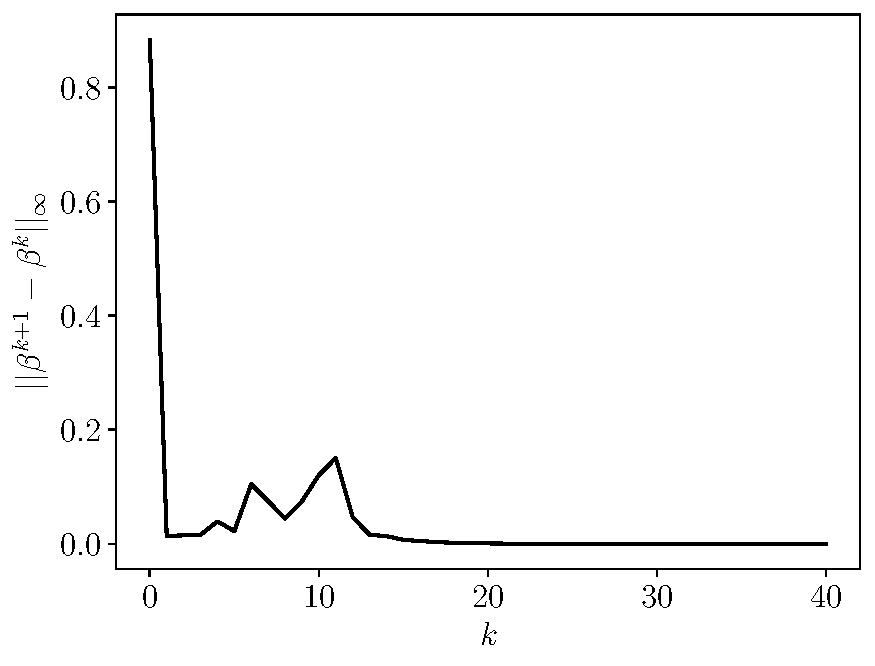
\includegraphics[scale=.5]{src/data}
  \end{figure}

    El código para remover outliers es:
    \inputminted[firstline=156]{python}{src/exam.py}

    Para esto se utilizaron tres matrices, la estimación usual, la estimación
    hecha por el método de Ledoit-Wolf y una estimación robusta usando Kendall.
    Las gráficas son:
    \begin{figure}[H]
      \centering
      \begin{subfigure}[b]{0.45\textwidth}
        \includegraphics[scale=.4]{src/cov-standard}
        \caption{Usual estimation.}
      \end{subfigure}
      %
      \begin{subfigure}[b]{0.45\textwidth}
        \includegraphics[scale=.4]{src/cov-lw}
        \caption{Ledoit-Wolf.}
      \end{subfigure}

      \begin{subfigure}[b]{0.45\textwidth}
        \includegraphics[scale=.4]{src/cov-kendall}
        \caption{Kendall.}
      \end{subfigure}
      %
      \begin{subfigure}[b]{0.45\textwidth}
        \includegraphics[scale=.4]{src/cov-oas}
        \caption{OAS.}
      \end{subfigure}
    \end{figure}
    Específicamente, para estos datos no se nota diferencia significativa entre
    ninguno de los 4 métodos. Se podrían intentar con otros métodos tales como
    otro Shrinkages, FastMCD, Pearon y etc.
\end{enumerate}
\end{document}
